\section{Results}

\subsection{Computational Environment}

The GRASP, Tabu, and Greedy algorithms were implemented in the Java programming language (Java version 17 and gradle version 7). The Integer Linear Programming was solved using Gurobi 9.5 and Python.

All the experiments were executed in a ideapad S145 81S90005BR: Lenovo IdeaPad S145 Notebook Intel Core i5-8265U (6MB Cache, 1.6GHz), 8GB DDR4-SDRAM, 460 GB SSD, Intel UHD Graphics 620.

The operating system was a Fedora 35 executando o Java 17 e Gradle 7. O código desenvolvido pode ser encontrado em \cite{bib:github}.

\subsection{Tables}

\begin{landscape}

\begin{table}
\centering
\begin{tabular}{lrrrrrrrrrrr}
\toprule
name & \multicolumn{3}{l}{problem\_info} & \multicolumn{2}{l}{ilp} & \multicolumn{2}{l}{greedy} & \multicolumn{2}{l}{grasp} & \multicolumn{2}{l}{tabu} \\
{} &     capacity & edges & nodes & cost &   time[s] &   cost & time[s] &  cost & time[s] & cost & time[s] \\
problem          &              &       &       &      &           &        &         &       &         &      &         \\
\midrule
N100\_E0\_W51666   &        51666 &     0 &   100 &   72 &  0.001373 &     69 &   0.008 &    70 &   0.031 &   70 &   0.025 \\
N100\_E0\_W52398   &        52398 &     0 &   100 &   72 &  0.002125 &     69 &   0.039 &    69 &   0.126 &   69 &   0.102 \\
N100\_E111\_W52365 &        52365 &   111 &   100 &   71 &  0.002847 &     70 &   0.009 &    70 &   0.025 &   70 &   0.044 \\
N100\_E118\_W52247 &        52247 &   118 &   100 &   71 &  0.003379 &     70 &   0.017 &    71 &   0.043 &   70 &   0.078 \\
N100\_E213\_W52199 &        52199 &   213 &   100 &   70 &  0.006474 &     70 &   0.006 &    70 &   0.014 &   69 &   0.056 \\
N100\_E222\_W53297 &        53297 &   222 &   100 &   70 &  0.011230 &     69 &   0.002 &    69 &   0.014 &   69 &   0.036 \\
\bottomrule
\end{tabular}
\caption{Cost and running time of all metaheuristics for problem instances with 100 nodes.}
\label{table:100-results}
\end{table}

\end{landscape}

\begin{landscape}

\begin{table}
\centering
\begin{tabular}{lrrrrrrrrrrr}
\toprule
name & \multicolumn{3}{l}{problem\_info} & \multicolumn{2}{l}{ilp} & \multicolumn{2}{l}{greedy} & \multicolumn{2}{l}{grasp} & \multicolumn{2}{l}{tabu} \\
{} &     capacity & edges & nodes & cost &   time[s] &   cost & time[s] &  cost & time[s] & cost & time[s] \\
problem            &              &       &       &      &           &        &         &       &         &      &         \\
\midrule
N500\_E570\_W262641  &       262641 &   570 &   500 &  361 &  0.010798 &    355 &   0.129 &   355 &   1.729 &  353 &   1.086 \\
N500\_E594\_W262931  &       262931 &   594 &   500 &  360 &  0.017267 &    353 &   0.127 &   356 &   1.524 &  353 &   1.040 \\
N500\_E598\_W263031  &       263031 &   598 &   500 &  359 &  0.024541 &    353 &   0.245 &   354 &   1.985 &  353 &   1.712 \\
N500\_E1157\_W262412 &       262412 &  1157 &   500 &  357 &  0.065347 &    351 &   0.072 &   353 &   0.595 &  352 &   1.046 \\
N500\_E1169\_W262155 &       262155 &  1169 &   500 &  356 &  0.061799 &    350 &   0.036 &   353 &   0.583 &  351 &   1.016 \\
N500\_E1189\_W260774 &       260774 &  1189 &   500 &  357 &  0.056502 &    353 &   0.058 &   353 &   0.621 &  351 &   0.990 \\
\bottomrule
\end{tabular}
\caption{Cost and running time of all metaheuristics for problem instances with 500 nodes.}
\label{table:500-results}
\end{table}

\end{landscape}

\begin{landscape}

\begin{table}
\centering
\begin{tabular}{lrrrrrrrrr}
\toprule
name & \multicolumn{3}{l}{problem\_info} & \multicolumn{2}{l}{greedy} & \multicolumn{2}{l}{grasp} & \multicolumn{2}{l}{tabu} \\
{} &     capacity & edges & nodes &   cost & time[s] &  cost & time[s] & cost & time[s] \\
problem             &              &       &       &        &         &       &         &      &         \\
\midrule
N1000\_E954\_W523944  &       523944 &   954 &  1000 &    707 &   1.311 &   710 &  27.659 &  707 &   8.613 \\
N1000\_E975\_W523980  &       523980 &   975 &  1000 &    708 &   0.702 &   712 &  22.837 &  712 &   7.913 \\
N1000\_E1017\_W523215 &       523215 &  1017 &  1000 &    708 &   0.751 &   711 &  22.985 &  708 &   8.659 \\
N1000\_E1925\_W523221 &       523221 &  1925 &  1000 &    706 &   0.489 &   707 &  10.759 &  703 &   7.565 \\
N1000\_E1956\_W527027 &       527027 &  1956 &  1000 &    705 &   0.549 &   708 &  10.030 &  705 &   7.726 \\
N1000\_E2032\_W526397 &       526397 &  2032 &  1000 &    706 &   0.235 &   708 &   7.158 &  701 &   6.929 \\
\bottomrule
\end{tabular}
\caption{Cost and running time of all metaheuristics for problem instances with 1000 nodes.}
\label{table:1000-results}
\end{table}

\end{landscape}


\subsection{Performance Profiles}

For those, a tolerance of 1\% is admitted in the solution. In other words, if an algorithms found a solution as good as the best one found (within a 1\% tolerance), then it is considered that it solved the problem in that run.

\begin{figure}[H]
    \centering
    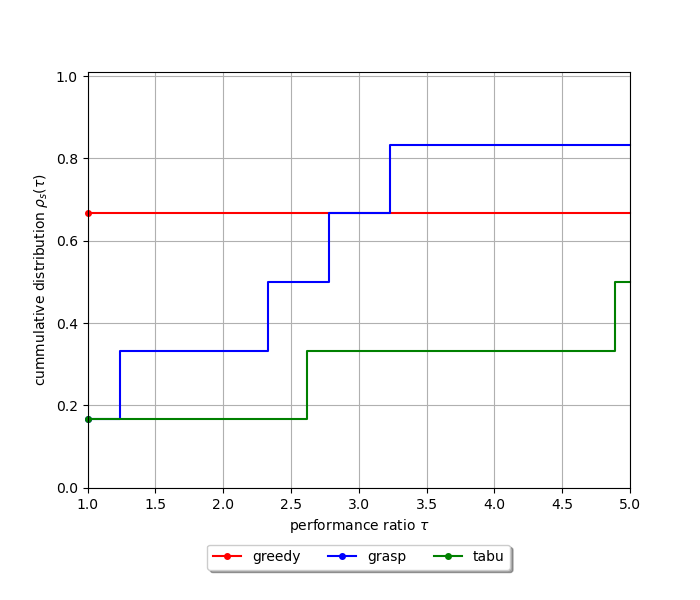
\includegraphics[width=\textwidth]{images/performance_profile/100_thmax_5.0.png}
    \caption{Performance Profiles for the three algorithms for the instances of 100 vertices.}
    \label{fig:perf-100}
\end{figure}

\begin{figure}[H]
    \centering
    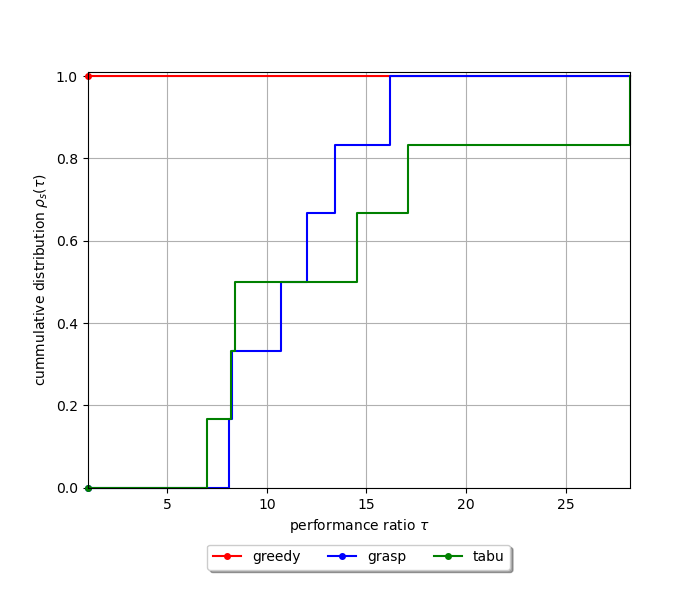
\includegraphics[width=\textwidth]{images/performance_profile/500_thmax_None.png}
    \caption{Performance Profiles for the three algorithms for the instances of 500 vertices.}
    \label{fig:perf-500}
\end{figure}


\begin{figure}[H]
    \centering
    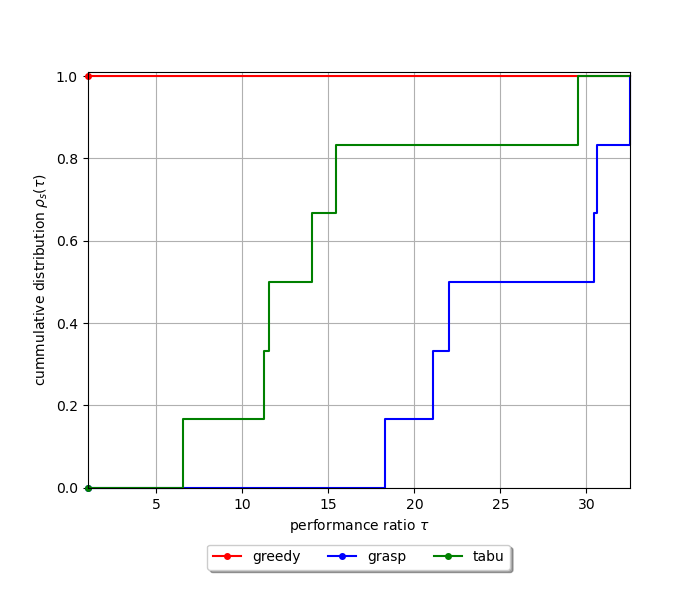
\includegraphics[width=\textwidth]{images/performance_profile/1000_thmax_None.png}
    \caption{Performance Profiles for the three algorithms for the instances of 1000 vertices.}
    \label{fig:perf-1000}
\end{figure}
